\documentclass[12pt]{article}
\usepackage[a4paper, top=2.5cm, bottom=1.25cm, left=3.5cm, right=1.25cm]{geometry}
\usepackage{newtxtext}
\usepackage{graphicx}
\usepackage{enumitem}
\usepackage{cite}   % improves citation formatting
\usepackage{url}    % handles URLs safely
\usepackage{setspace}
\usepackage{float}
\usepackage{setspace}

\usepackage{fancyhdr}

\pagestyle{fancy}
\fancyhf{}                    % Clear header and footer

% Page number centered and slightly raised
\fancyfoot[C]{\raisebox{12pt}{\thepage}}

\renewcommand{\headrulewidth}{0pt}
\renewcommand{\footrulewidth}{0pt}
\begin{document}
\pagenumbering{roman}
\begin{titlepage}
    \centering
    \thispagestyle{empty}
    
    {\fontsize{24pt}{28pt}\selectfont \bfseries
    BLOCKCHAIN SECURE VAULT {\fontsize{12pt}{14pt}\selectfont } \par}
    \vspace{0.9cm}
    
    {\fontsize{14pt}{18pt}\selectfont \bfseries
    MINOR PROJECT REPORT {\fontsize{12pt}{14pt}\selectfont } \par}
    \vspace{1.2cm}
    
    {\fontsize{12pt}{14pt}\selectfont
    SUBMITTED IN PARTIAL FULFILMENT OF THE REQUIREMENTS FOR THE AWARD OF THE DEGREE OF {\fontsize{12pt}{14pt}\selectfont }\par}
    \vspace{1.4cm}
    
    {\fontsize{14pt}{18pt}\selectfont 
    \textbf{BACHELOR OF TECHNOLOGY} \\
    {\fontsize{14pt}{18pt}\selectfont{Computer Science and Engineering}} {\fontsize{12pt}{14pt}\selectfont } 
    \par}
    \vspace{1.9cm}
    
    
\includegraphics[width=0.35\textwidth]{gne_logo.png}\par
    \vspace{1.9cm}
    
    {\fontsize{14pt}{18pt}\selectfont
    \noindent
    \begin{minipage}[t]{0.69\textwidth}
        \raggedright
        \textbf{Submitted By:} \\
        Ekampreet Singh \hspace{0.2cm}(2302515) {\fontsize{12pt}{14pt}\selectfont } \\
        Gaurav Prashar \hspace{0.2cm}(2302518) {\fontsize{12pt}{14pt}\selectfont } \\
        Gaurav Sharma \hspace{0.2cm}(2302519) {\fontsize{12pt}{14pt}\selectfont } \\
    \end{minipage}%
    \hfill
    \begin{minipage}[t]{0.29\textwidth}
        \textbf{Submitted To:} \\ 
        Er. Meetali \\
        \textit{Assistant Professor} \\
    \end{minipage}}
    
    \vspace{1.9cm}
    
    {\fontsize{14pt}{18pt}\selectfont \bfseries
    DEPARTMENT OF COMPUTER SCIENCE AND ENGINEERING\\
    GURU NANAK DEV ENGINEERING COLLEGE\\
    LUDHIANA, 141006 {\fontsize{12pt}{14pt}\selectfont } \par}
    
    \vspace{0.5cm}
    {\fontsize{12pt}{14pt}\selectfont MAY, 2026 \par}
    
\end{titlepage}
\newpage


\begin{abstract}
\doublespacing
Blockchain Secure Document Vault is a trustless document management system that integrates end-to-end encryption, decentralized storage, and blockchain-based integrity verification. The platform addresses critical limitations of centralized cloud storage solutions by enabling organizations operating in compliance-intensive sectors such as legal, healthcare, and finance to maintain complete control over document security while generating immutable proof of file integrity and access history.

The system follows a hybrid architecture in which documents are encrypted locally using the AES-256 encryption standard and hashed using the SHA-256 algorithm. Encrypted files are stored on the InterPlanetary File System (IPFS) to ensure decentralized availability, while cryptographic integrity hashes are committed to a blockchain ledger to provide tamper-proof verification. Users retain full ownership of cryptographic keys, ensuring a trustless security model, while benefiting from a transparent and verifiable audit trail that reduces reliance on manual compliance audits.

The technology stack includes Next.js and React for the frontend, Node.js with Express and MongoDB for backend services, Solidity-based smart contracts for integrity proofs, and IPFS for distributed storage. The project has been fully developed and tested, achieving stable performance and secure operation, making it suitable for real-world deployment.
\end{abstract}

\newpage
\begin{center}
    {\fontsize{16pt}{18pt}\selectfont\textbf{ACKNOWLEDGEMENT}}
\end{center}

\begin{spacing}{1.5}

\noindent I/We are highly grateful to Dr. Sehijpal Singh, Principal, Guru Nanak Dev Engineering College (GNDEC), Ludhiana, for providing this opportunity to carry out the minor project work. The constant guidance and encouragement received from Dr. Kiran Jyoti, H.O.D. CSE Department, GNDEC Ludhiana, has been of great help in carrying out the project work and is acknowledged with reverential thanks. I/We would like to express a deep sense of gratitude and thanks profusely to Er. Meetali, Assisstant Professor; without his/her wise counsel and able guidance, it would have been impossible to complete the project in this manner. I/We express gratitude to other faculty members of the Computer Science and Engineering Department of GNDEC for their intellectual support throughout the course of this work. Finally, I/We are indebted to all who have contributed to this report work.

\end{spacing}

\vspace{0.5cm}

\noindent{\fontsize{12pt}{14pt}\selectfont\textbf{Ekampreet Singh}}\\

\noindent{\fontsize{12pt}{14pt}\selectfont\textbf{Gaurav Prashar}}\\

\noindent{\fontsize{12pt}{14pt}\selectfont\textbf{Gaurav Sharma}}\\

\newpage

\tableofcontents
\newpage
\listoffigures
\newpage

\clearpage

% Main matter
\pagenumbering{arabic}
\setcounter{page}{1}
\newpage
\section{Introduction}

\subsection{Project Overview}

This project presents a secure and user-friendly platform for document storage with verifiable integrity. Conventional cloud storage solutions often prioritize convenience over security, leading to risks related to confidentiality and undetectable tampering \cite{stallings2017}. To overcome these limitations, the proposed system integrates end-to-end encryption with blockchain-based verification, ensuring that documents remain private while their authenticity can be independently validated.

Users can securely register, upload encrypted documents, and verify file integrity by comparing cryptographic hashes with immutable on-chain records. A modern web interface, combined with a robust backend, manages encryption, access control, and secure sharing workflows\cite{conti2018}. The system aims to make strong security practices and trustworthy document verification accessible to individuals and organizations without requiring specialized expertise.

\subsection{Technology Used}

\begin{itemize}
\item \textbf{Frontend:} Next.js with TypeScript
\item \textbf{Backend:} Node.js and Express for REST APIs, authentication, and file handling
\item \textbf{Blockchain:} Solidity smart contracts using Hardhat for on-chain hash storage and verification
\item \textbf{Cryptography:} AES-256 for encryption and SHA-256 for hashing \cite{nist197}
\item \textbf{File Processing:} Mammoth.js for DOCX files, PDF.js for PDF rendering, and Web Crypto API for client-side decryption
\end{itemize}

\subsection{Field of Project}

\begin{itemize}
\item Information Security and Web Application Development
\item Blockchain-based Integrity Verification\cite{dorri2017}
\item Secure and Compliance-Oriented Document Management
\end{itemize}

\subsection{Special Technical Terms}

\begin{itemize}
\item \textbf{End-to-End Encryption (E2EE):} Files are encrypted before upload and decrypted only by authorized users.
\item \textbf{Content Hash:} A cryptographic fingerprint used to detect file modifications.
\item \textbf{On-chain Verification:} Validation of file integrity using immutable blockchain records.
\item \textbf{Smart Contract:} Blockchain program that stores and exposes document hashes.\cite{ijraset2021}
\item \textbf{Immutable Ledger:} Tamper-resistant blockchain record ensuring data integrity.
\end{itemize}

\subsection{Objectives of the Project}

The primary objectives of the proposed system are as follows:

\begin{enumerate}
\item To design and deploy smart contracts on a blockchain platform for storing SHA-256 document hashes, ensuring immutability and transparency of records.
\item To encrypt documents using the AES-256 encryption standard and store the encrypted files on IPFS to provide secure and decentralized storage.
\item To develop a secure document management dashboard that allows users to upload, view, verify, and download documents through a browser-based interface.
\item To implement a verification mechanism that allows users to confirm the authenticity and integrity of documents by comparing their cryptographic hashes with blockchain records.
\end{enumerate}\newpage
\section{Requirement Analysis and System Specification}

\subsection{Problem Definition}

Organizations and individuals need a way to store sensitive documents so they are confidential, tamper-evident, and easy to verify later. Traditional cloud storage can protect availability, but it does not natively provide immutable proof of document authenticity. The required system is a secure document vault that encrypts files, stores encrypted payloads off-chain, and records document fingerprints on blockchain for trustable verification.


\subsection{Identity \& Access Module}

\begin{itemize}
\item User registration and login (password, Google, OTP).
\item Email verification with OTP before full access.
\item JWT-based session management, protected APIs, logout/token invalidation.
\item Profile retrieval and access control for user-owned resources.
\end{itemize}

\subsection{Secure Document Processing Module}

\begin{itemize}
\item File intake with validation (type/size checks).
\item Hash generation (SHA-256) for integrity identity.
\item AES-256 encryption before external storage.
\item Encrypted upload to decentralized/object storage and metadata persistence.
\item Key-handling rule: decryption key shown once to user, not stored server-side.
\end{itemize}

\subsection{Blockchain Integrity Module}

\begin{itemize}
\item Smart contract stores mapping of file hash $\rightarrow$ storage reference.
\item On upload: record hash transaction and persist transaction reference.
\item On verify: recompute hash from uploaded file and compare with on-chain record.
\item Return authenticity status (verified / not found / mismatch) with audit-ready metadata.
\end{itemize}

\subsection{Sharing \& Retrieval Module}

\begin{itemize}
\item Owner can share document access with registered recipients.
\item Recipient can view/download encrypted content with out-of-band decryption key.
\item Owner can revoke active share access.
\item Document dashboard for ``my documents,'' ``shared with me,'' and ``shared by me.''
\end{itemize}

\subsection{Key Non-Functional Requirements}

\begin{itemize}
\item \textbf{Security:} Encryption at rest, strict authentication checks, and minimal secret exposure.
\item \textbf{Reliability:} Graceful handling of blockchain, IPFS, or service failures.
\item \textbf{Performance:} Responsive upload and verification flows for typical file sizes.
\item \textbf{Usability:} Simple workflows for upload, key copying, verification, sharing, and revocation.
\end{itemize}

This section describes the hardware and software requirements necessary to develop and run the Blockchain Secure Document Vault system.

\subsection{Hardware Requirements}

\begin{center}
\begin{tabular}{|l|p{10cm}|}
\hline
\textbf{Component} & \textbf{Requirement} \\
\hline
Processor & Intel Core i3 (8th Generation) / AMD Ryzen 3 or higher \\
\hline
RAM & Minimum 4 GB (Recommended 8 GB) \\
\hline
Storage & Minimum 2 GB free disk space (Recommended SSD with at least 10 GB free space) \\
\hline
Network & Stable internet connection for blockchain interaction, IPFS storage, and email OTP services \\
\hline
\end{tabular}
\end{center}

\subsection{Software Requirements}

\begin{center}
\begin{tabular}{|l|p{10cm}|}
\hline
\textbf{Software} & \textbf{Requirement} \\
\hline
Operating System & Windows 10/11, Linux, or macOS \\
\hline
Code Editor & Visual Studio Code \\
\hline
Runtime Environment & Node.js (v18 or higher) \\
\hline
Backend Framework & Express.js \\
\hline
Frontend Framework & Next.js (React with TypeScript) \\
\hline
Database & MongoDB \\
\hline
Blockchain Development & Hardhat and Ethers.js \\
\hline
API Testing Tool & Postman \\
\hline
Version Control & Git and GitHub \\
\hline
\end{tabular}
\end{center}

\subsection{Browser Requirements}

\begin{center}
\begin{tabular}{|l|p{10cm}|}
\hline
\textbf{Browser} & \textbf{Requirement} \\
\hline
Google Chrome & Latest Version \\
\hline
Microsoft Edge & Latest Version \\
\hline
JavaScript & Must be enabled \\
\hline
\end{tabular}
\end{center}

\newpage
\section{System Design}

This section presents the detailed design of the Blockchain Secure Document Vault system. The design addresses all four objectives defined in the project synopsis and explains how each objective is technically achieved.

\subsection{Design Approach Overview}

The system follows a hybrid architecture combining:

\begin{itemize}
\item Blockchain (for immutability and transparency)
\item IPFS (for decentralized encrypted file storage)
\item AES-256 encryption (for confidentiality)
\item Web-based dashboard (for secure interaction)
\end{itemize}

The architecture ensures that:

\begin{itemize}
\item Documents remain confidential
\item Hash records remain immutable
\item Verification remains transparent
\item Users maintain ownership and access control
\end{itemize}

\subsection{Objective 1: Smart Contract for SHA-256 Hash Storage (Immutability \& Transparency)}

To ensure tamper-proof document verification, a smart contract named \texttt{DocumentStorage} is deployed on the blockchain.\cite{ijarsct2022}

\textbf{Design Details:}

When a user uploads a document:

\begin{itemize}
\item The system generates a SHA-256 hash of the original file.
\item The smart contract stores the following metadata:
\begin{itemize}
\item File Hash (bytes32)
\item IPFS CID
\item Owner Address
\item Timestamp
\end{itemize}
\end{itemize}

\textbf{Core Functions:}

\begin{itemize}
\item \texttt{storeDocumentHash(hash, ipfsCID)} \\ 
Stores document metadata and rejects duplicate hashes.

\item \texttt{verifyDocumentHash(hash)} \\ 
Returns whether the document exists and its associated metadata.
\end{itemize}

\textbf{Design Outcome:}

\begin{itemize}
\item Immutability is ensured because blockchain records cannot be altered.
\item Transparency is achieved because transaction hashes are publicly auditable.
\end{itemize}

\subsection{Objective 2: AES-256 Encryption and IPFS Decentralized Storage}

To maintain confidentiality and secure storage, the system encrypts documents before uploading them to IPFS.\cite{jisem2023}

\textbf{Design Steps:}

\begin{enumerate}
\item File is received by backend.
\item SHA-256 hash is generated.
\item File is encrypted using:
\begin{itemize}
\item AES-256 algorithm
\item Unique randomly generated key
\item Random Initialization Vector (IV)
\end{itemize}
\item Only encrypted file is uploaded to IPFS.
\item Plaintext file is never stored externally.
\end{enumerate}

\textbf{Security Rule:}

\begin{itemize}
\item The encryption key is displayed once to the user.
\item The server does not store the decryption key.
\end{itemize}

\textbf{Design Outcome:}

\begin{itemize}
\item Confidentiality is preserved.
\item Even if IPFS is accessed, the file remains unreadable.
\item Blockchain stores only the hash, not the file content.
\end{itemize}

\subsection{Objective 3: Secure Document Dashboard (View, Verify, Download)}

A secure web-based dashboard provides document management functionality.

\textbf{Features:}

\textbf{1. Upload}
\begin{itemize}
\item Upload file
\item Encryption and blockchain recording
\item Display transaction reference
\end{itemize}

\textbf{2. View}
\begin{itemize}
\item Fetch encrypted file from IPFS
\item Decrypt in browser using user key
\item Render preview
\end{itemize}

\textbf{3. Download}
\begin{itemize}
\item Retrieve encrypted file
\item Decrypt using provided key
\item Download original file
\end{itemize}

\textbf{4. Access Control}
\begin{itemize}
\item JWT-based authentication
\item Users can access only their own or shared documents
\item Revocation support for shared access
\end{itemize}

\textbf{Design Outcome:}

\begin{itemize}
\item Secure interaction
\item Controlled access
\item User-friendly interface
\end{itemize}

\subsection{Objective 4: Document Validity Verification}

The system provides a blockchain-based verification mechanism.\cite{arxiv2205}

\textbf{Verification Process:}

\begin{enumerate}
\item User uploads a file for verification.
\item System recomputes SHA-256 hash.
\item Smart contract verification function is called.
\end{enumerate}

If the hash exists:

\begin{itemize}
\item Document is marked authentic.
\item Blockchain transaction hash is shown.
\item Timestamp is displayed.
\end{itemize}

If not found:

\begin{itemize}
\item Document is marked invalid.
\end{itemize}

\textbf{Design Outcome:}

\begin{itemize}
\item Tamper-evident validation
\item Audit-ready proof
\item Trustable verification mechanism
\end{itemize}
\begin{figure}[H]
\centering
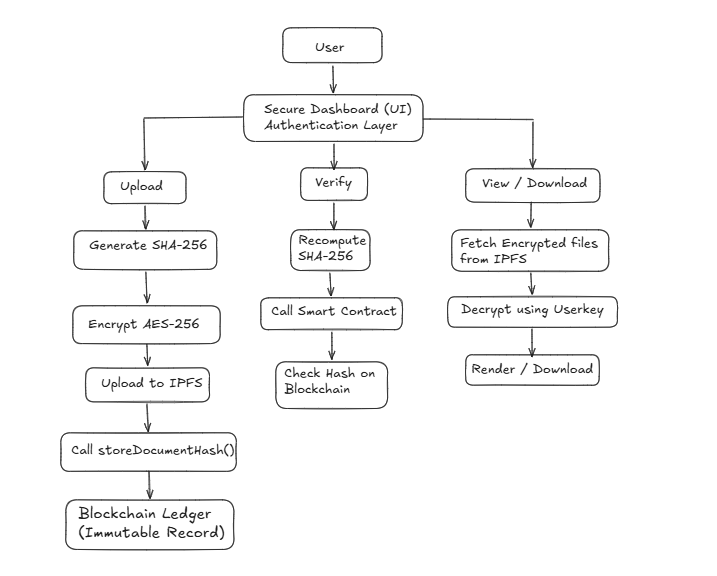
\includegraphics[width=15cm]{photos/flowChart.png}
\caption{Control flow of Blockchain Secure Vault}
\label{fig:flowchart}
\end{figure}
\newpage
\section{Implementation, Testing and Maintenance}

This section describes the testing techniques proposed for validating the Blockchain Secure Document Vault system. The objective of testing is to ensure correctness, security, reliability, and performance of all system components including smart contracts, backend services, encryption mechanisms, and dashboard functionality.

\subsection{Proposed Testing Techniques}

To ensure comprehensive system validation, the following testing strategies will be used.

\subsubsection{Unit Testing}

Unit testing is performed to validate individual components and functions independently.

\textbf{Modules Covered:}
\begin{itemize}
\item SHA-256 hashing function
\item AES-256 encryption and decryption
\item JWT authentication logic
\item OTP verification logic
\item Smart contract functions (\texttt{storeDocumentHash}, \texttt{verifyDocumentHash})
\end{itemize}

\textbf{Purpose:}  
To ensure each function performs accurately in isolation.

\subsubsection{Integration Testing}

Integration testing verifies interaction between connected modules.

\textbf{Interfaces Tested:}
\begin{itemize}
\item Backend API $\leftrightarrow$ Database (MongoDB)
\item Backend API $\leftrightarrow$ IPFS storage
\item Backend API $\leftrightarrow$ Blockchain smart contract
\item Dashboard $\leftrightarrow$ Backend API
\end{itemize}

\textbf{Purpose:}  
To confirm correct data flow and communication between system components.

\subsubsection{Smart Contract Testing}

Smart contract testing ensures on-chain correctness.

\textbf{Scenarios Tested:}
\begin{itemize}
\item Duplicate hash prevention
\item Correct storage of metadata
\item Accurate verification response
\item Transaction reversion on invalid operations
\end{itemize}

\textbf{Purpose:}  
To guarantee immutability and integrity of blockchain records.

\subsubsection{API Testing}

API endpoints are tested using tools such as Postman.

\textbf{Validation Includes:}
\begin{itemize}
\item Correct status codes (200, 401, 403, 409, 500)
\item Input validation
\item Error handling
\item Response format verification
\end{itemize}

\textbf{Purpose:}  
To ensure reliable backend services.

\subsubsection{Security Testing}

Security testing validates access control and protection mechanisms.

\textbf{Checks Include:}
\begin{itemize}
\item Unauthorized access denial
\item Invalid or expired JWT token rejection
\item Role-based access enforcement
\item Proper key-handling behavior (no server-side key storage)
\end{itemize}

\textbf{Purpose:}  
To protect against unauthorized access and data breaches.

\subsubsection{End-to-End (E2E) Testing}

Simulates real user workflows.

\begin{itemize}
\item Register $\rightarrow$ Verify OTP $\rightarrow$ Login
\item Upload $\rightarrow$ Encrypt $\rightarrow$ Store $\rightarrow$ Record on blockchain
\item Verify document authenticity
\item View and download document
\item Share and revoke access
\end{itemize}

\textbf{Purpose:}  
To validate complete system functionality under realistic scenarios.

\subsubsection{Performance and Load Testing}

System performance is evaluated under:

\begin{itemize}
\item Multiple concurrent uploads
\item Multiple verification requests
\item Large file uploads (within allowed limit)
\end{itemize}

\textbf{Purpose:}  
To measure system responsiveness and stability.

\subsubsection{Usability and Compatibility Testing}

Dashboard is tested on:

\begin{itemize}
\item Google Chrome
\item Mozilla Firefox
\item Microsoft Edge
\item Mobile and desktop viewports
\end{itemize}

\textbf{Purpose:}  
To ensure consistent user experience across platforms.

\subsection{System Test Cases}

The following test cases will be executed to validate system functionality.



\subsubsection{TC01 -- User Registration (Valid Case)} 
Input: Valid full name, username, email, password \newline
Expected Result: Account created, OTP sent, user marked as unverified.

\subsubsection{TC02 -- OTP Verification (Valid Case)} 
Input: Correct OTP within expiry period \newline
Expected Result: Email verified successfully and login permitted.

\subsubsection{TC03 -- Login (Invalid Password)} 
Input: Correct username with incorrect password \newline
Expected Result: 401 Unauthorized response, no JWT issued.

\subsubsection{TC04 -- Access Protected API Without Token} 
Input: Request to secured endpoint without JWT \newline
Expected Result: 401 Unauthorized error.

\subsubsection{TC05 -- Upload Valid File} 
Input: Supported file (e.g., PDF within size limit) \newline
Expected Result:
\begin{itemize}
\item SHA-256 generated
\item AES-256 encryption completed
\item File uploaded to IPFS
\item Hash recorded on blockchain
\item Decryption key displayed once
\end{itemize}

\subsubsection{TC06 -- Upload Duplicate File} 
Input: Same file uploaded again \newline
Expected Result: Upload rejected with duplicate error; no second blockchain entry created.

\subsubsection{TC07 -- Upload Unsupported File Type} 
Input: Unsupported extension \newline
Expected Result: Validation failure with appropriate error message.

\subsubsection{TC08 -- Verify Authentic Document} 
Input: Previously uploaded original file \newline
Expected Result: Hash matches blockchain record; document marked as verified.

\subsubsection{TC09 -- Verify Tampered or Unknown Document} 
Input: Modified file or never-uploaded file \newline
Expected Result: Verification fails; document marked invalid or not found.

\subsubsection{TC10 -- Dashboard View (Correct Key)} 
Input: Valid document with correct decryption key \newline
Expected Result: Successful decryption and document preview.

\subsubsection{TC11 -- Dashboard View (Incorrect Key)} 
Input: Valid document with wrong decryption key \newline
Expected Result: Decryption fails; file not rendered.

\subsubsection{TC12 -- Download Document (Authorized)} 
Input: Valid key for owned/shared document \newline
Expected Result: Original decrypted file downloaded successfully.

\subsubsection{TC13 -- Unauthorized Document Access} 
Input: User attempts to access unshared document \newline
Expected Result: 403 Forbidden or 404 Not Found response.

\subsubsection{TC14 -- Share Document} 
Input: Owner shares document with valid registered user\newline
Expected Result: Share record created; recipient can access document.

\subsubsection{TC15 -- Revoke Shared Access} 
Input: Owner revokes access \newline
Expected Result: Recipient can no longer view or download document.

\subsubsection{TC16 -- Smart Contract Immutability Check} 
Input: Attempt to overwrite existing hash \newline
Expected Result: Transaction reverted; original data unchanged.

\subsubsection{TC17 -- IPFS or Service Failure Handling} 
Input: Simulated IPFS unavailability \newline
Expected Result: Graceful error response; no inconsistent records created.

\subsubsection{TC18 -- Expired or Blacklisted Token} 
Input: Expired or invalid JWT token \newline
Expected Result: Request denied; user redirected to login.

\subsection{Maintenance}

The Blockchain Secure Document Vault requires continuous maintenance to ensure security, reliability, and usability after deployment.

\subsubsection{System Monitoring}
The Blockchain Secure Document Vault should be continuously monitored to ensure smooth operation. Server performance, storage usage, blockchain transaction logs, and API responses should be checked regularly. Monitoring tools can help detect unusual activities or failures in real time.

\subsubsection{Security Maintenance}
Since the project deals with sensitive documents, security maintenance is critical. This includes:

\begin{itemize}
    \item Regular updating of cryptographic libraries
    \item Periodic security audits
    \item Smart contract vulnerability testing
    \item Access control verification
    \item Patch management for dependencies
\end{itemize}

Private keys and encryption keys should be stored securely and rotated periodically.

\subsubsection{Database and Storage Maintenance}
The decentralized storage system such as InterPlanetary File System (IPFS) or cloud backup services should be monitored for data availability and integrity. Backup copies of metadata and configuration files should be maintained to prevent accidental loss.

\subsubsection{Blockchain Network Maintenance}
The blockchain network requires regular maintenance to ensure efficient transaction processing. This includes:

\begin{itemize}
    \item Monitoring gas fees
    \item Checking node synchronization
    \item Updating blockchain client software
    \item Monitoring smart contract execution
\end{itemize}

If deployed on platforms such as Ethereum, network upgrades should be tracked and integrated when necessary.

\subsubsection{Software Updates}
Application components including frontend, backend, APIs, and blockchain libraries should be updated regularly to fix bugs, improve performance, and add new features. Version control systems such as GitHub can be used to manage updates efficiently.


\subsubsection{User Support and Access Management}
User accounts should be reviewed periodically. Inactive accounts should be disabled, and user permissions should be updated according to organizational requirements. Password reset and wallet recovery mechanisms should also be maintained.

\subsubsection{Performance Optimization}
System performance should be evaluated periodically by analyzing:

\begin{itemize}
    \item Transaction speed
    \item File upload/download time
    \item Encryption/decryption performance
    \item Network latency
\end{itemize}

Optimization techniques should be applied whenever performance degradation is observed.

\subsubsection{Bug Fixing and Documentation}
Any bugs reported by users should be logged, analyzed, and fixed promptly. Technical documentation, API documentation, and user manuals should be updated after every major change.

\subsubsection{Scalability Planning}
As the number of users and documents increases, infrastructure should be scaled accordingly. Additional nodes, storage capacity, and load balancing mechanisms may be introduced to maintain system efficiency.

\subsubsection{Compliance and Audit}
Regular compliance checks and audit trails should be maintained to ensure transparency, accountability, and adherence to data security standards.


\newpage

\section{Results and Discussion}

The Blockchain Secure Document Vault was successfully developed and tested to provide secure, decentralized document storage and verification. The system integrates encryption, decentralized storage, and blockchain technology to ensure confidentiality, integrity, and transparency of stored documents.

\subsection{User Registration and Authentication}
The system successfully allows users to register and authenticate using secure credentials and email/password authentication, Google authentication, and OTP-based authentication. Only authorized users can access their stored documents, ensuring access control and security.

\begin{figure}[H]
\centering
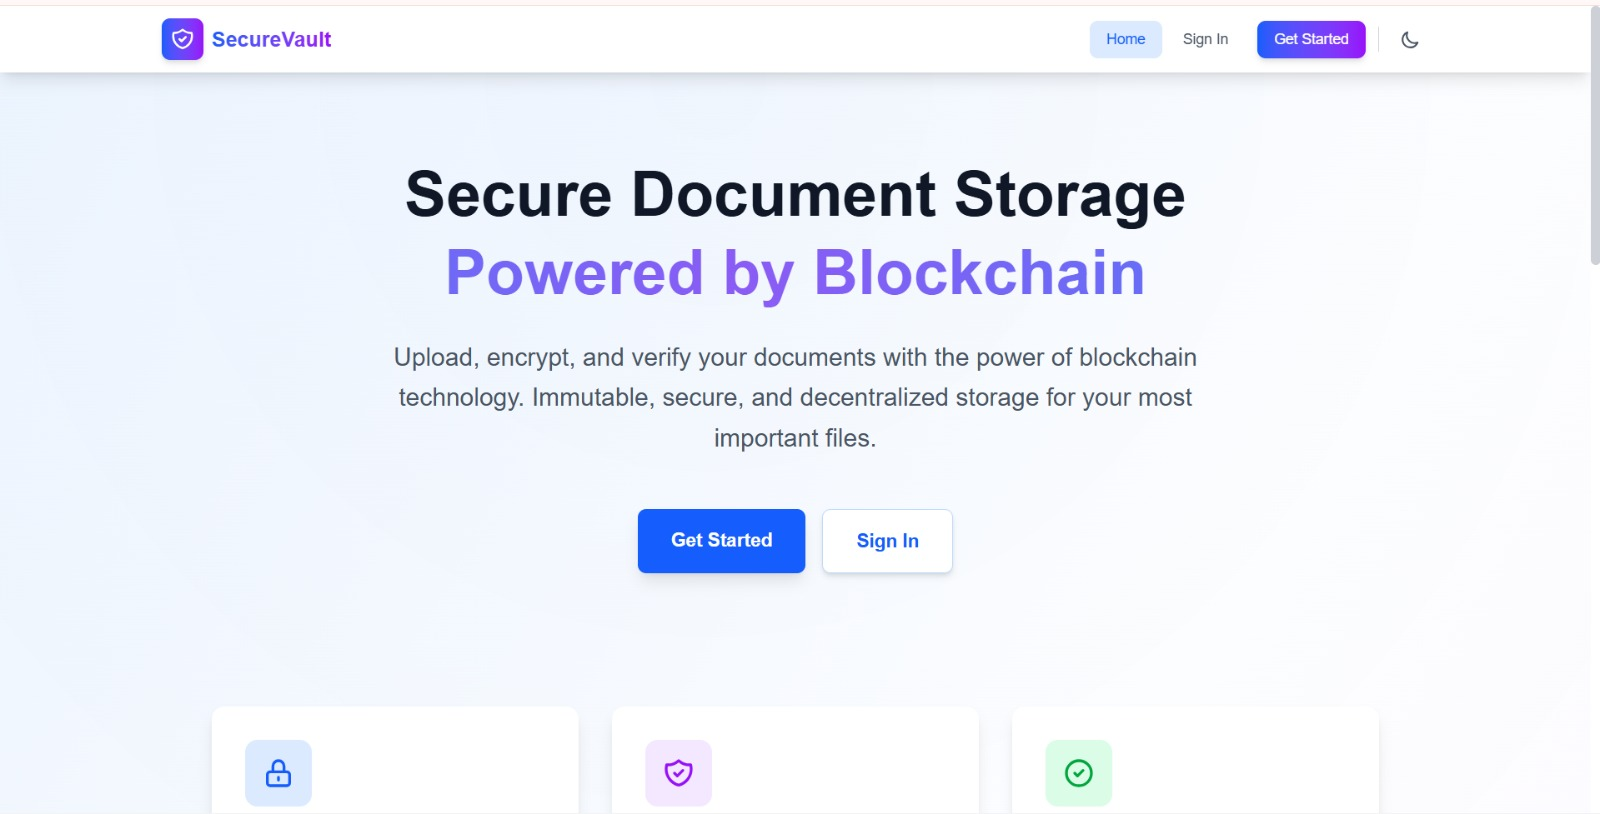
\includegraphics[width=15cm]{photos/one.jpeg}
\caption{Landing page of the system before user authentication}
\label{fig:one}
\end{figure}

\begin{figure}[H]
\centering
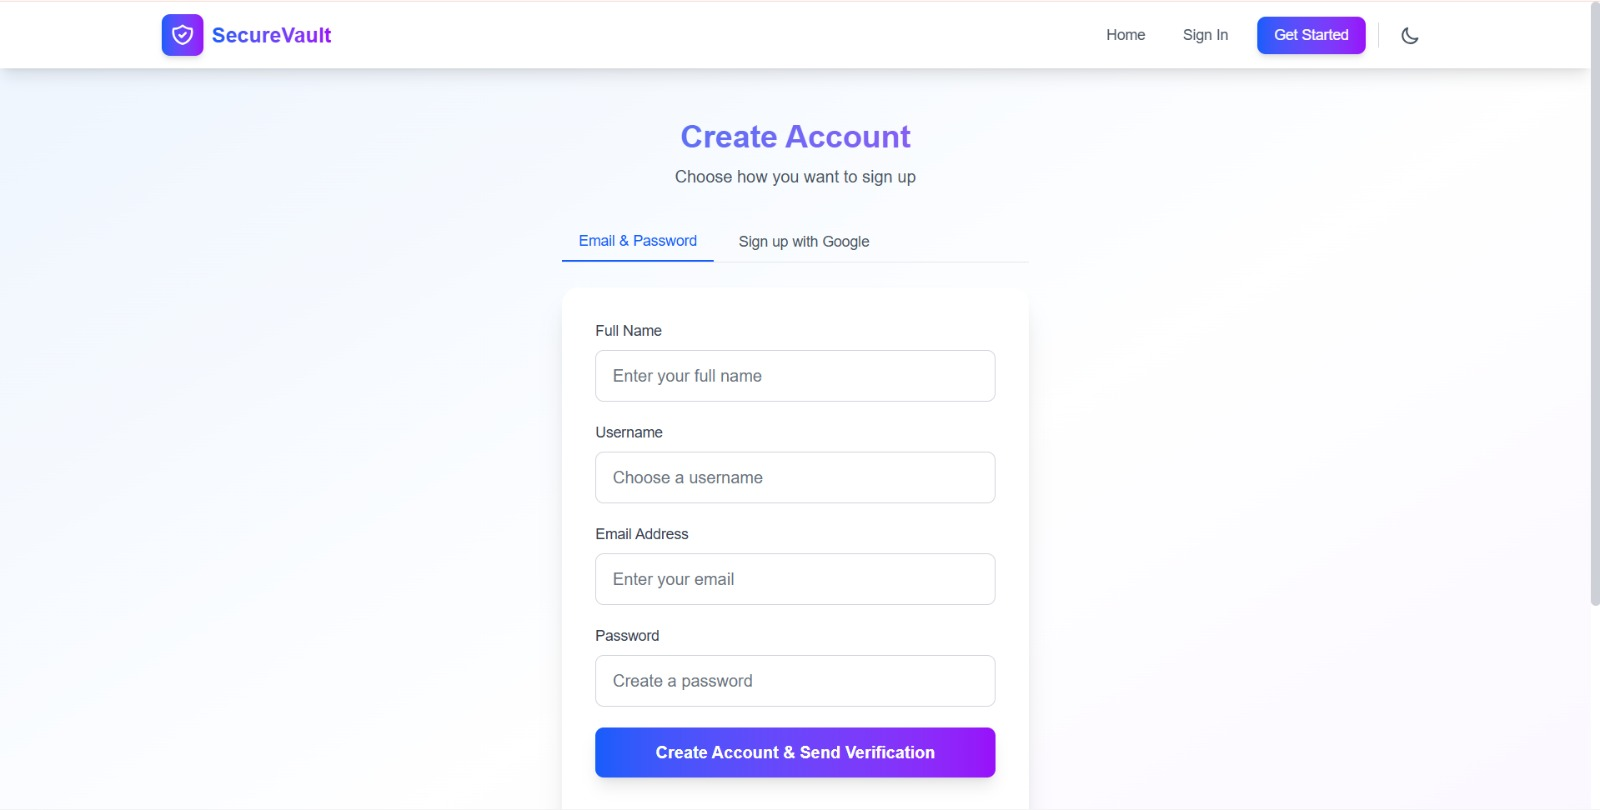
\includegraphics[width=15cm]{photos/two.jpeg}
\caption{User registration interface for creating a new account}
\label{fig:two}
\end{figure}

\begin{figure}[H]
\centering
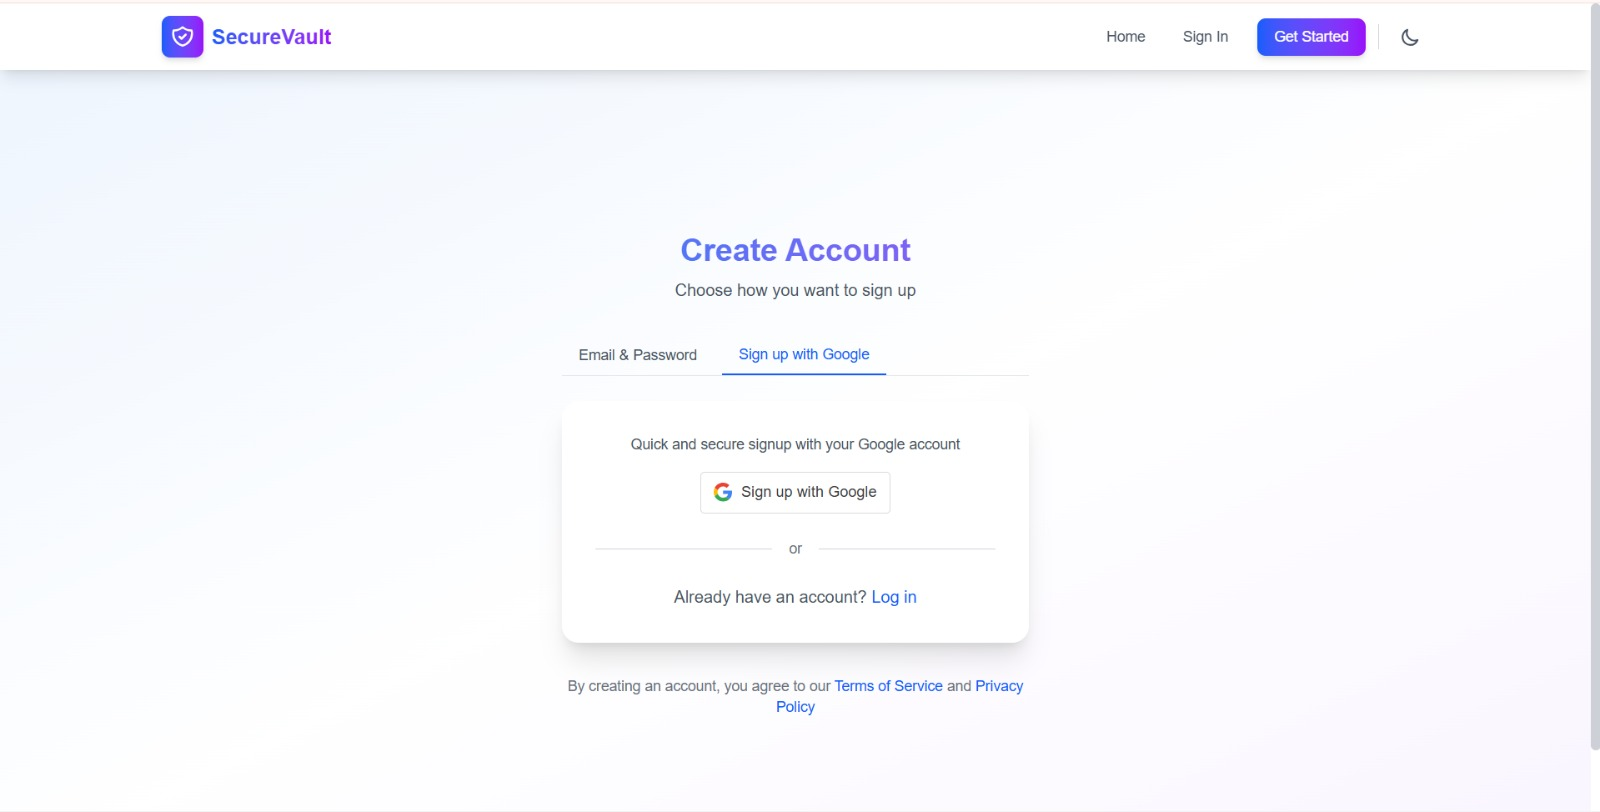
\includegraphics[width=15cm]{photos/three.jpeg}
\caption{Account registration using Google authentication}
\label{fig:three}
\end{figure}

\begin{figure}[H]
\centering
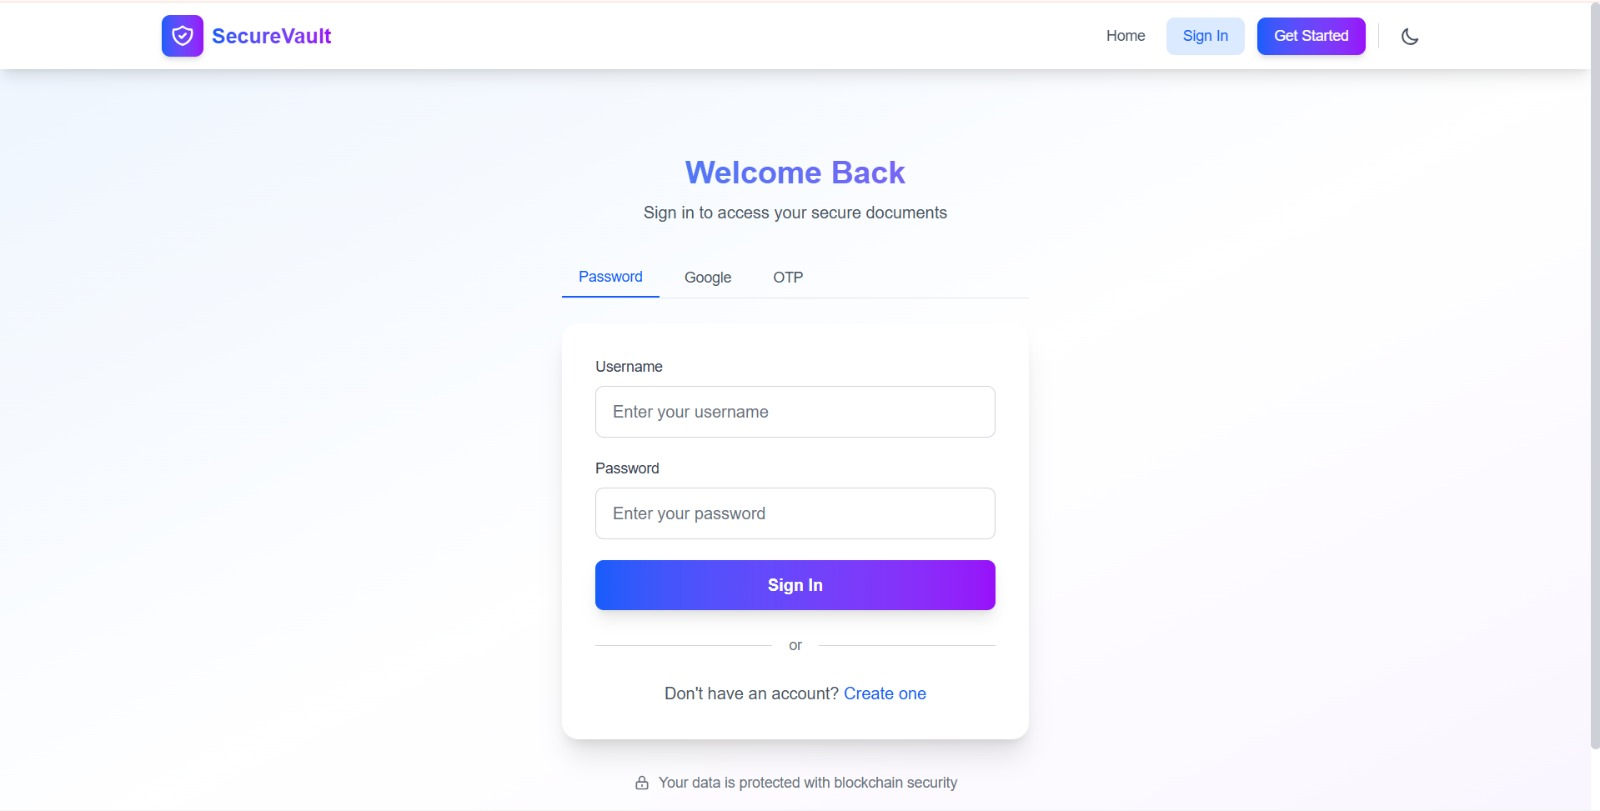
\includegraphics[width=15cm]{photos/four.jpeg}
\caption{User login interface using username and password}
\label{fig:four}
\end{figure}

\begin{figure}[H]
\centering
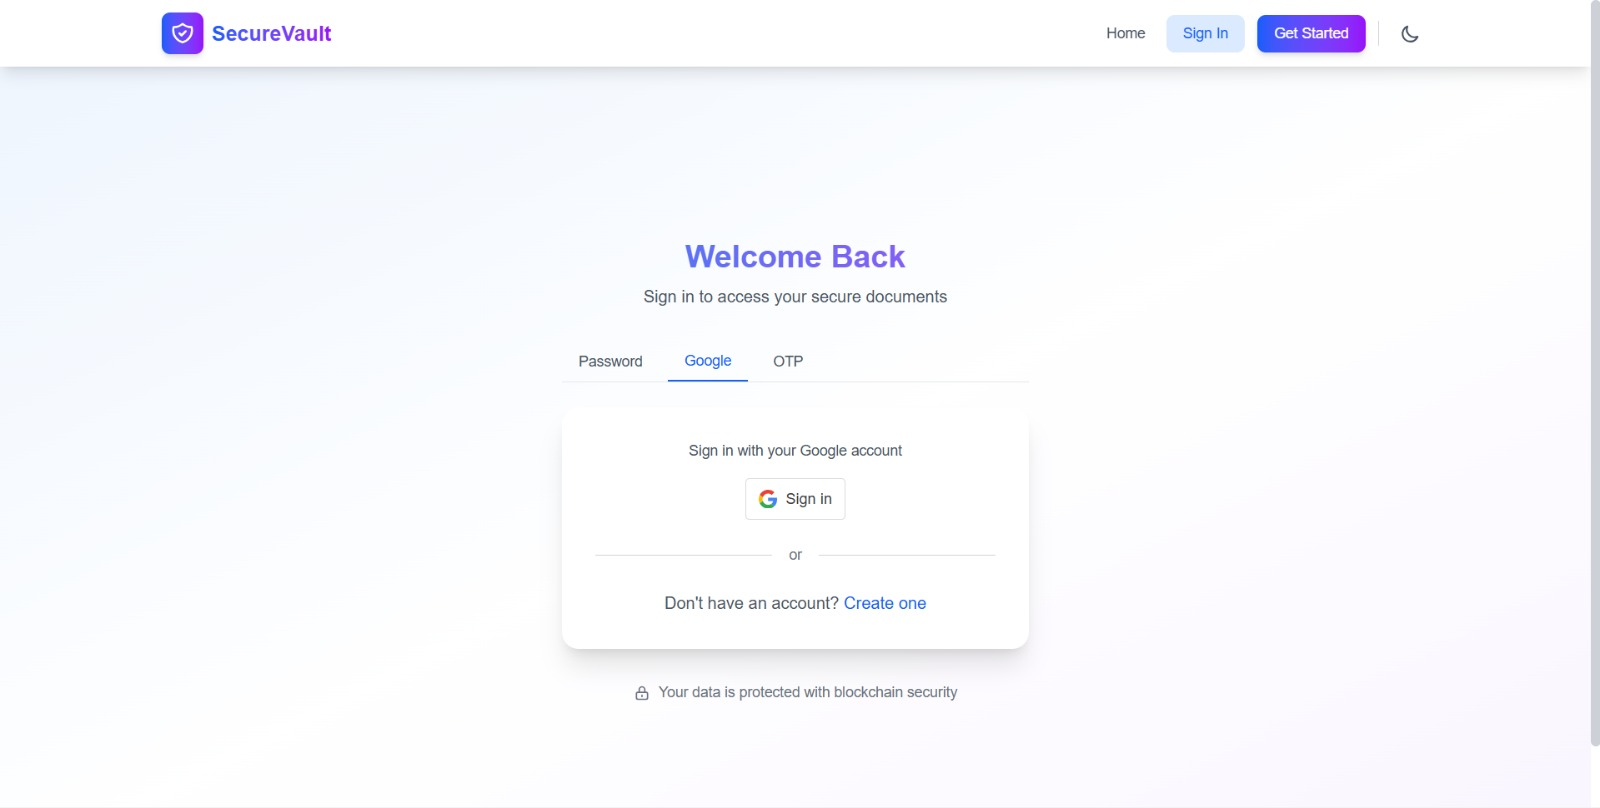
\includegraphics[width=15cm]{photos/five.jpeg}
\caption{User login using Google authentication}
\label{fig:five}
\end{figure}

\begin{figure}[H]
\centering
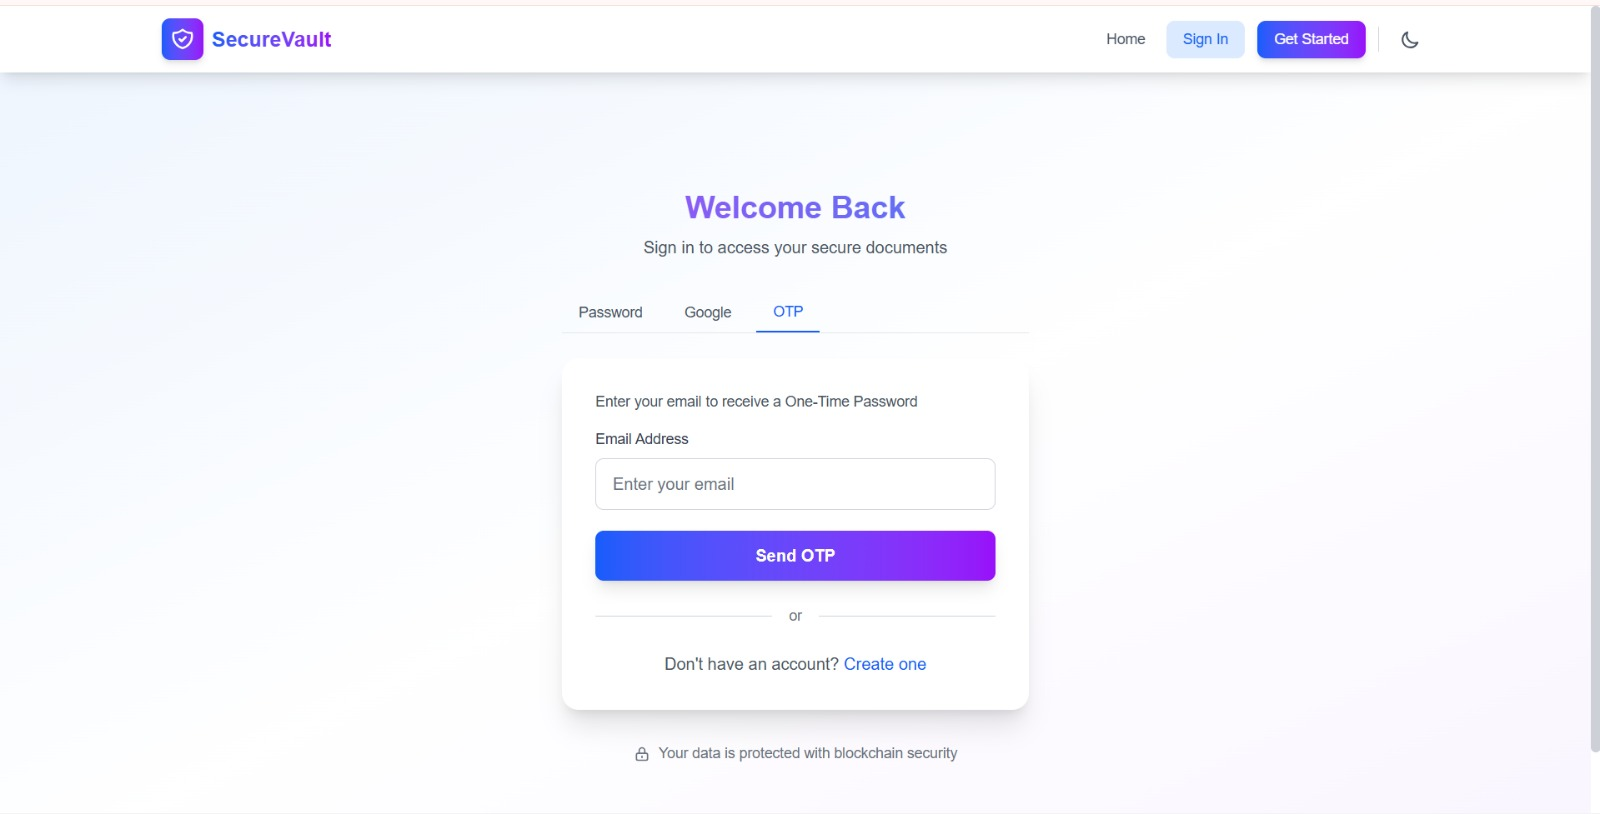
\includegraphics[width=15cm]{photos/six.jpeg}
\caption{User login using One-Time Password (OTP) verification}
\label{fig:six}
\end{figure}

\begin{figure}[H]
\centering
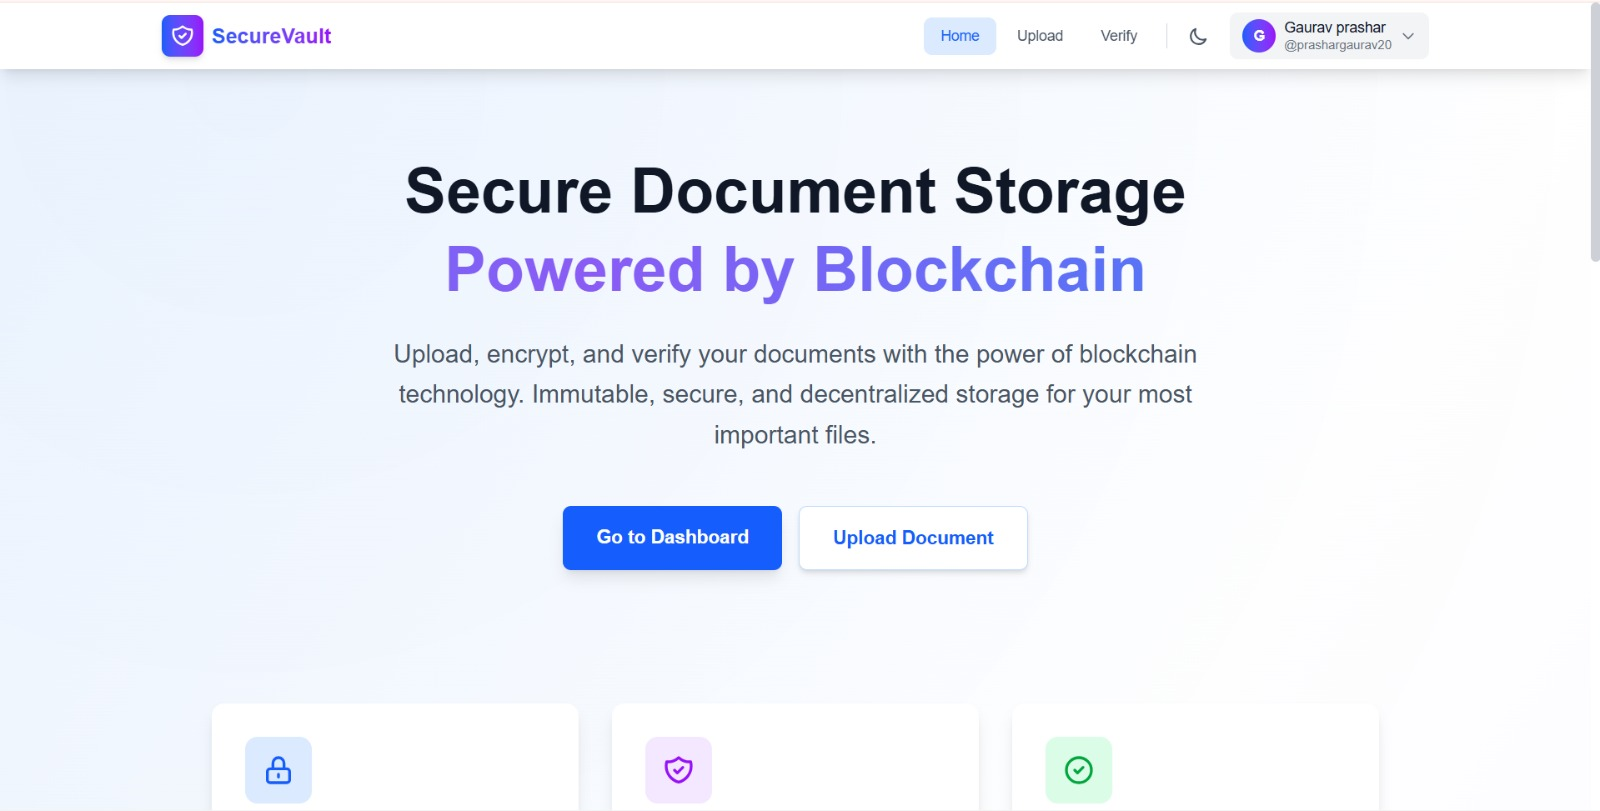
\includegraphics[width=15cm]{photos/nine.jpeg}
\caption{Home interface displayed after user authentication}
\label{fig:nine}
\end{figure}


\subsection{Secure Document Upload}
Users were able to upload documents successfully. Each uploaded document was encrypted before storage, ensuring confidentiality of sensitive data.

\begin{figure}[H]
\centering
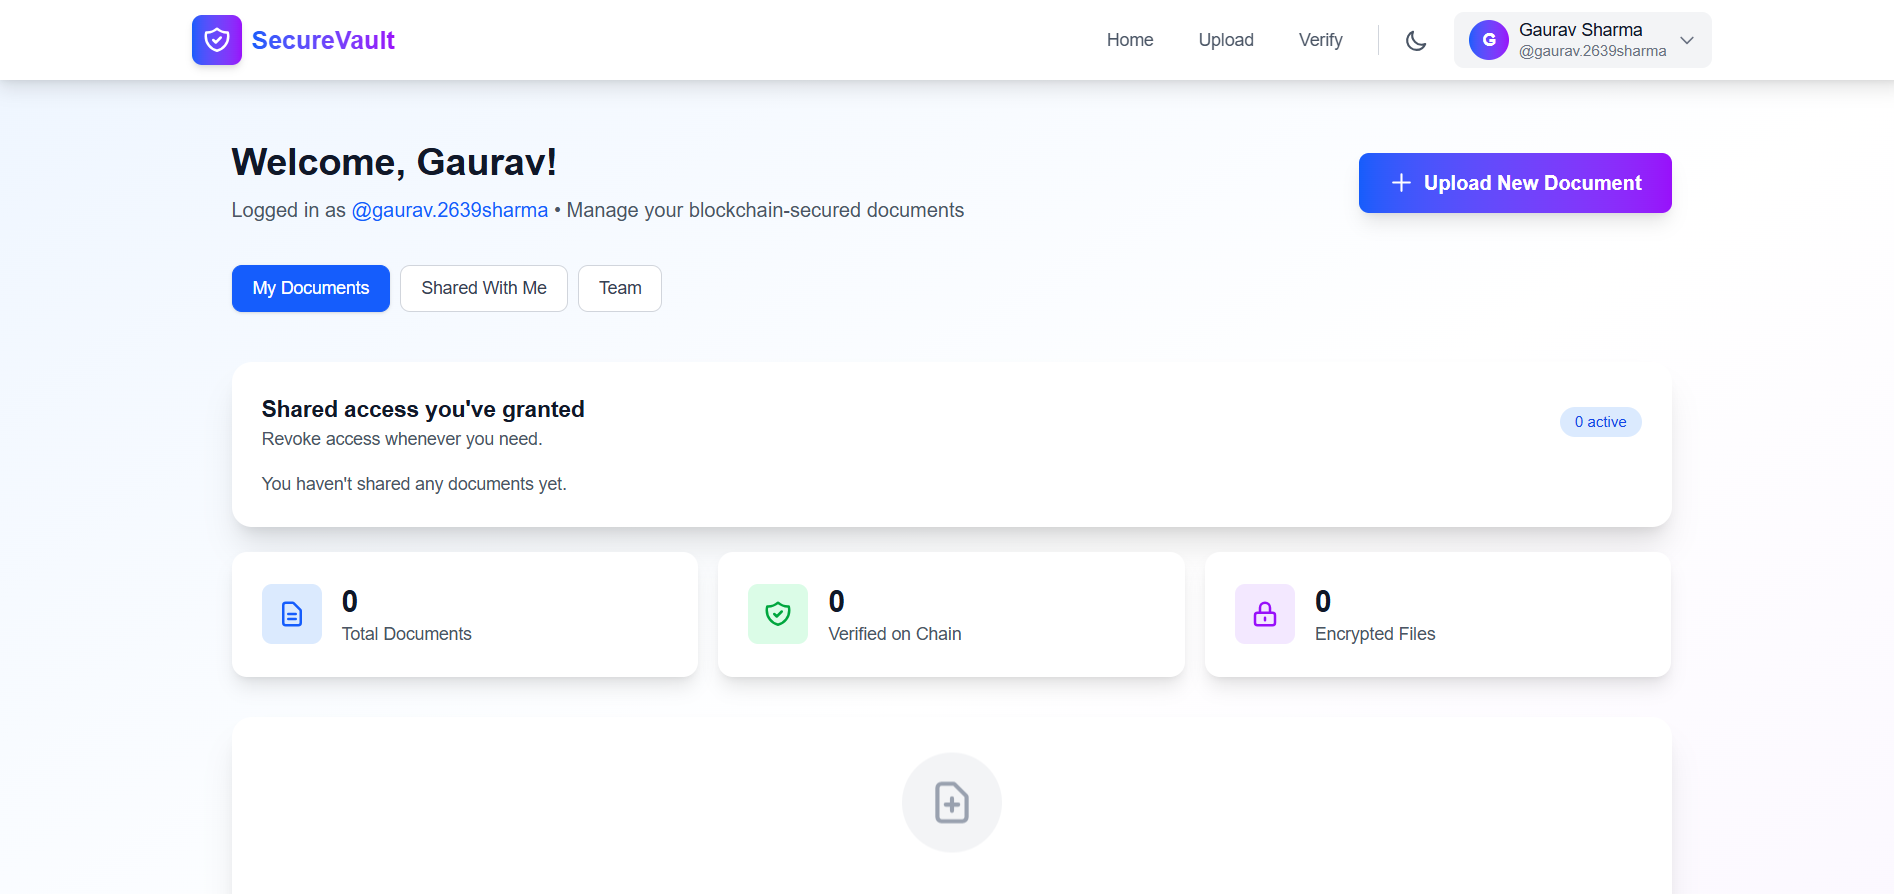
\includegraphics[width=15cm]{photos/eight.png}
\caption{Secure document management dashboard after successful login}
\label{fig:eight}
\end{figure}

\begin{figure}[H]
\centering
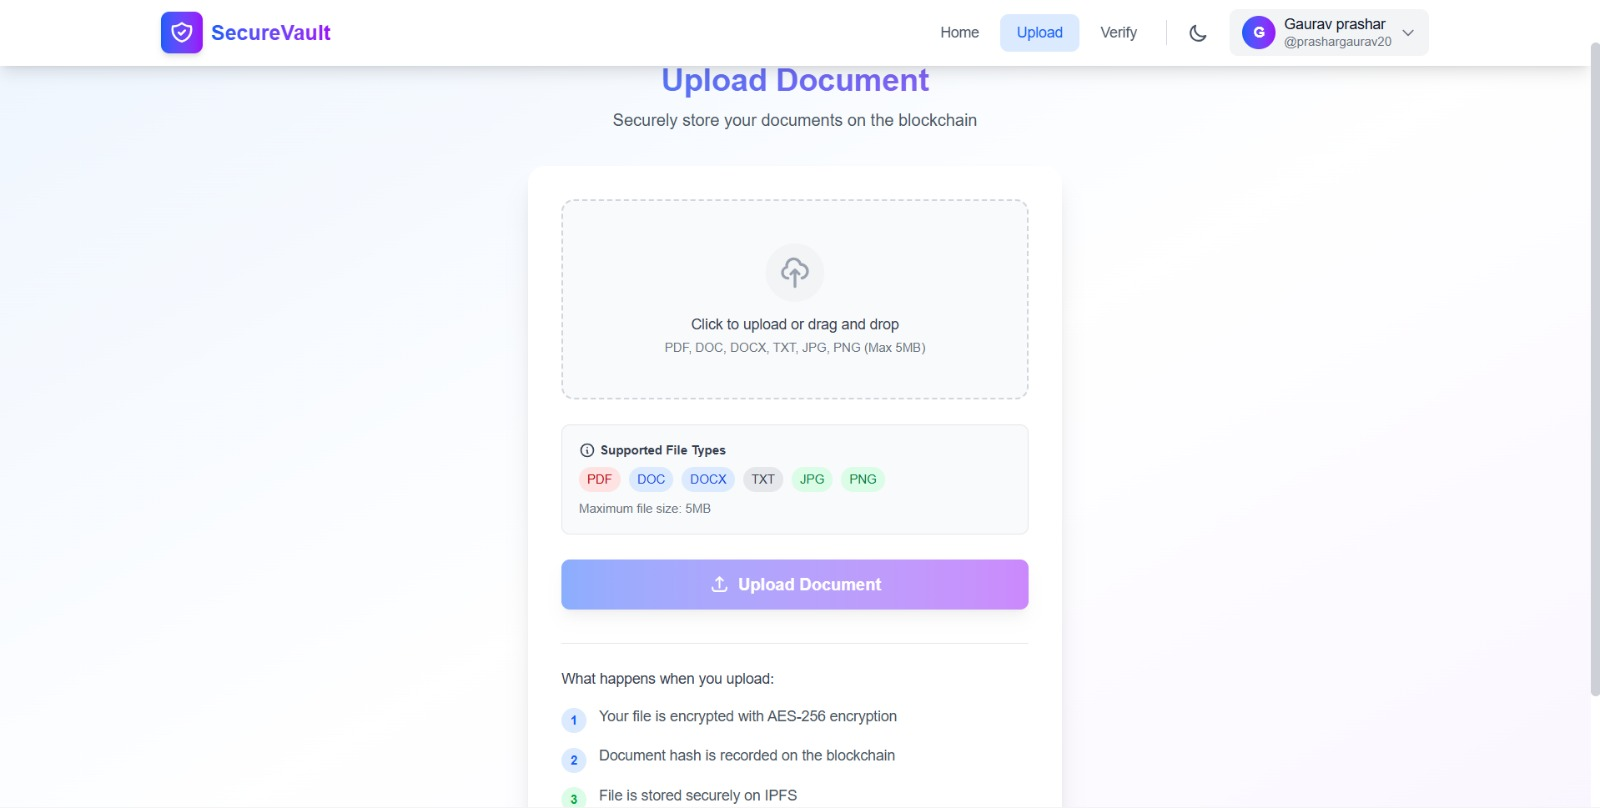
\includegraphics[width=15cm]{photos/ten.jpeg}
\caption{Document upload interface for secure file encryption and storage}
\label{fig:ten}
\end{figure}

\begin{figure}[H]
    \centering
    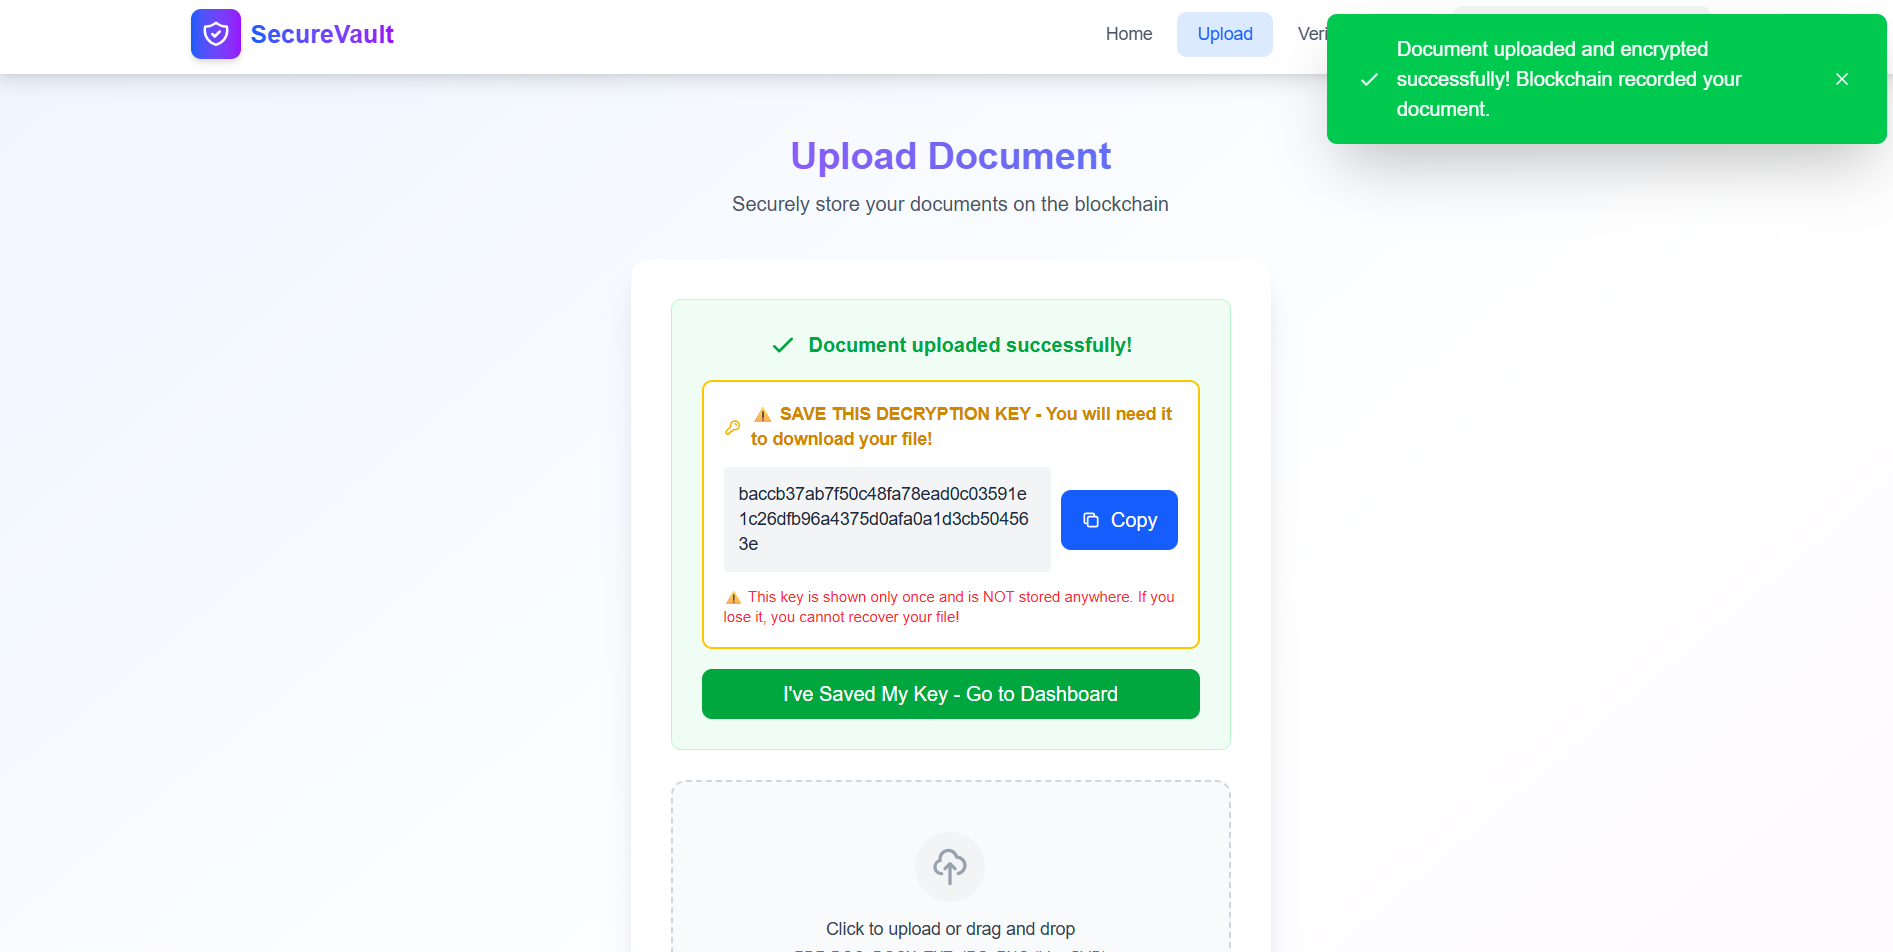
\includegraphics[width=15cm]{photos/upload.png} 
    \caption{Secure Document Upload with IPFS and Pinata Integration}
    \label{fig:ten}
\end{figure}

\subsection{Decentralized Storage}
Uploaded documents were securely stored using the InterPlanetary File System (IPFS) integrated with Pinata. Each uploaded file generated a unique content-based hash (CID), ensuring data integrity, tamper resistance, and efficient decentralized retrieval. By leveraging Pinata’s pinning services, the files remained persistently available on the IPFS network while maintaining reliable accessibility and secure storage.

\subsection{Blockchain-Based Verification}
Document hashes were successfully recorded on the blockchain network. The system verified document authenticity by comparing stored hashes with generated hashes, preventing tampering and unauthorized modification.

\begin{figure}[H]
\centering
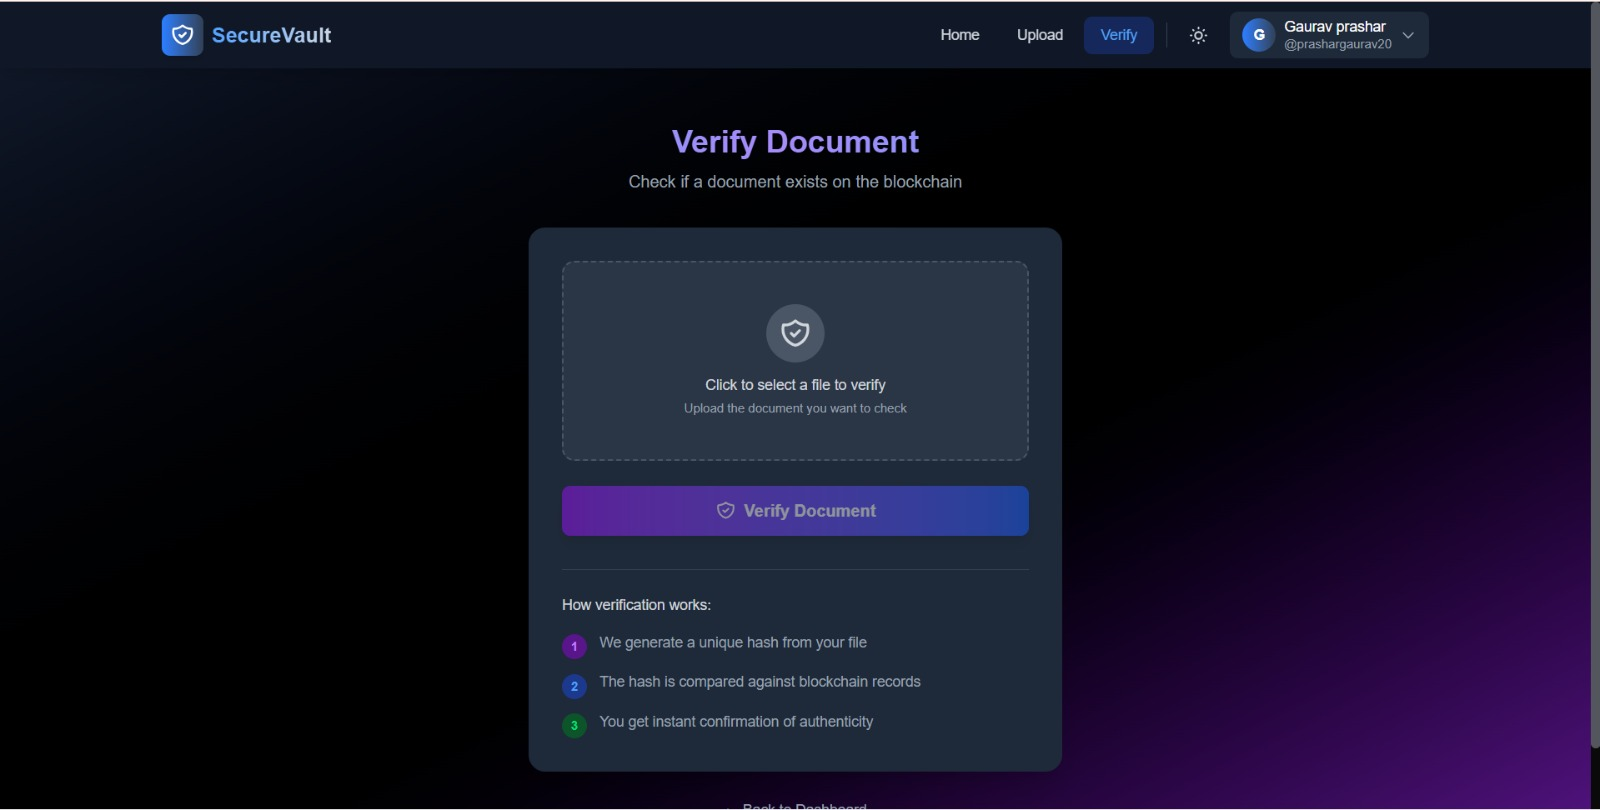
\includegraphics[width=15cm]{photos/eleven.jpeg}
\caption{Document verification interface for validating file authenticity using blockchain records}
\label{fig:eleven}
\end{figure}

\begin{figure}[H]
    \centering
    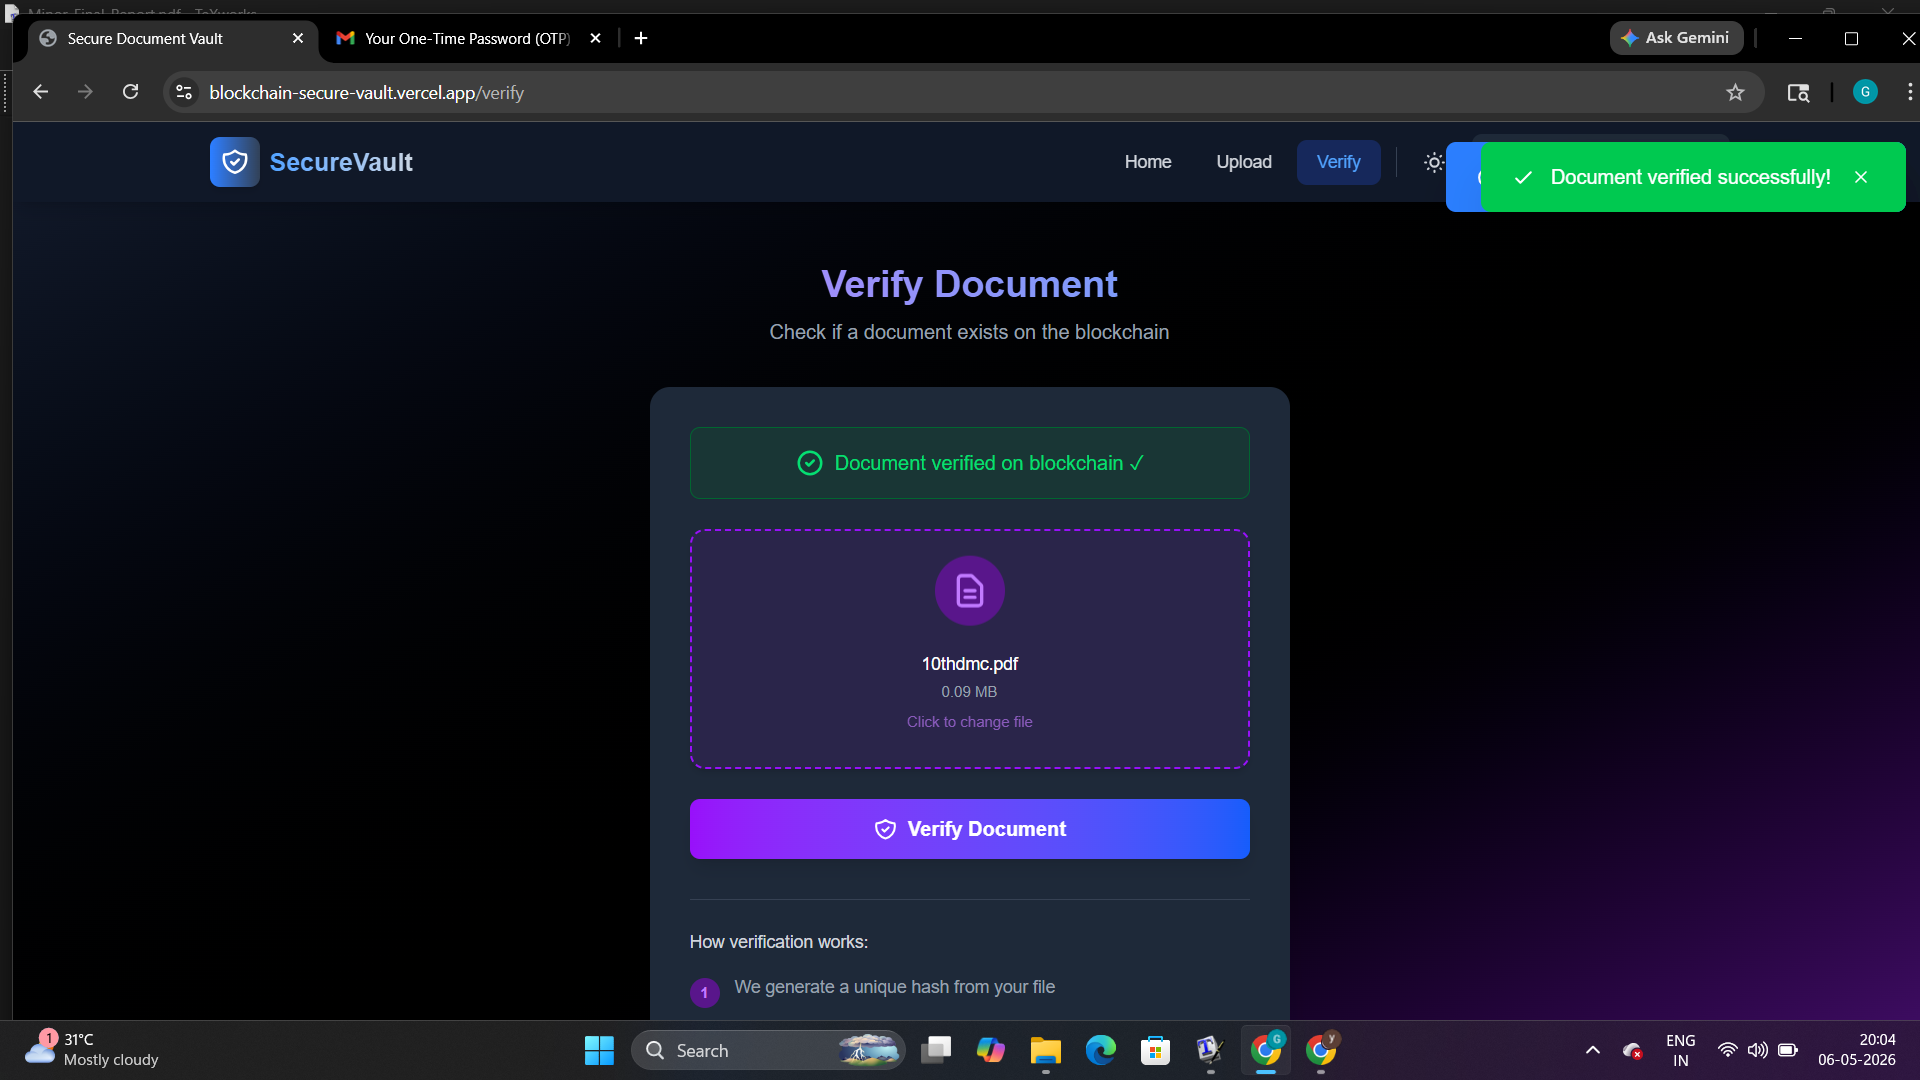
\includegraphics[width=15cm]{photos/verify.png}
    \caption{Document Integrity Verified Successfully}
    \label{fig:ten}
\end{figure}

\subsection{Retrieval and Decryption}
Authorized users successfully retrieved and decrypted stored documents. The retrieval process maintained data integrity and confidentiality throughout the operation.



\subsection{Performance Analysis}
The system was tested under different workloads, and the following observations were made:

\begin{itemize}
    \item File upload and retrieval were completed successfully.
    \item Blockchain transactions were executed correctly.
    \item Smart contract interactions were reliable.
    \item Encryption and decryption operations introduced minimal computational overhead.
\end{itemize}

\subsection{Security Analysis}
The implemented system demonstrated strong resistance against common security threats such as:

\begin{itemize}
    \item Unauthorized access
    \item Data tampering
    \item Centralized storage failure
    \item Integrity compromise
\end{itemize}

\subsection{Discussion}
The experimental results show that blockchain technology combined with encryption and decentralized storage provides a reliable solution for secure document management. Compared to traditional centralized systems, the developed system offers improved transparency, immutability, and user control. Although blockchain transaction latency and gas costs may affect scalability, the system successfully achieves its primary objective of secure and trustworthy document storage.

\newpage
\section{Conclusion and Future Scope}

\subsection{conclusion}
The Blockchain Secure Document Vault successfully demonstrates a secure, decentralized, and trustless approach to document management. By integrating end-to-end encryption, decentralized storage, and blockchain-based verification, the system addresses the major limitations of traditional centralized storage solutions, particularly in terms of data integrity, transparency, and user control. The implementation leverages strong cryptographic standards such as AES-256 for data confidentiality and SHA-256 for integrity assurance, combined with decentralized storage using InterPlanetary File System and blockchain-based immutability. This hybrid architecture ensures that sensitive documents remain secure while providing verifiable proof of authenticity and access history. The developed system has been thoroughly tested and demonstrates stable performance, scalability, and robustness. It enables users to maintain full ownership of their cryptographic keys, ensuring a trustless environment without reliance on centralized authorities. Overall, the project validates the practical applicability of blockchain and decentralized technologies in enhancing document security and compliance, making it suitable for deployment in real-world, compliance-intensive environments.

\subsection{future scope}
Although the current system provides a strong foundation for secure and decentralized document management, several enhancements can be explored to further improve functionality, scalability, and usability.Future work may include the integration of advanced key management solutions such as multi-signature authentication and hardware wallet support to further strengthen security. The incorporation of zero-knowledge proof mechanisms can enhance privacy by enabling verification without revealing sensitive information. Integration with enterprise systems and cloud platforms can improve adoption in large-scale organizational environments. Furthermore, enhancing the user interface and experience using modern frameworks like Next.js can make the system more accessible to non-technical users. Finally, future development may focus on regulatory compliance features, cross-chain interoperability, and mobile application support, enabling broader adoption across industries such as healthcare, legal services, and finance.











\newpage

\bibliographystyle{IEEEtran}
\bibliography{references}

\end{document}
